\setchapterstyle{lines}
\labch{appendix}
%%\blinddocument

\chapter{Caso de Estudio: Tecnología Web}
\label{sec:caso-estudio-A}

La Web es un sistema abierto que se  caracteriza por \sidecite{Couloris2011}: a) Su funcionamiento está basado en estándares de comunicación y contenido o en documentos que se publican e implementan libremente. Ejemplo, hay varios tipos de navegador,  implementado en distintas plataformas; así como  implementaciones de servidores web. b) La Web está abierta con respecto a los tipos de \gls{recursos} que se pueden publicar y compartir. Los navegadores están diseñados para adaptarse a nuevas funcionalidades de presentación de contenido en forma de aplicaciones auxiliares y complementos o \textit{plug-ins}.

La Web se basa en  componentes tecnológicos que son  estándares de la W3C, \sidecite{W3C2022} y que se describen en esta parte. Se presentan una introducción a las siguientes tecnolog\'ias que se usan  en la web: HTTP, HTML, CCS, JavaScript.
 
\section{HTTP}   \index{HTTP}
	 HTTP (HyperText Transfer Protocol), \gls{HTTP} es el protocolo usado cuando se visita cualquier sitio web desde un navegador (\textit{browser}). Es un protocolo confiable que facilita la transferencia de información en la web. Esta característica de fiabilidad es  debido a que HTTP utiliza protocolos de transmisión de datos confiables, garantiza que sus datos no se dañarán ni se codificarán durante el tránsito, incluso cuando provengan del otro lado del mundo \sidecite{W3C2022}, \sidecite{Gourley2002},  \sidecite{Allen2017}.

\begin{description}
	\item[Clientes y Servidores Web]
	El contenido de la  web está almacenado en \gls{servidores web}. Los servidores web usan el protocolo HTTP, por lo que a menudo se les llama servidores HTTP. Estos servidores almacenan los datos de Internet y proporcionan los datos cuando los solicitan los clientes HTTP. Los clientes envían solicitudes HTTP a los servidores y los servidores devuelven los datos solicitados en respuestas HTTP, como se muestra en la Figura \ref{fig:CSweb} . 
	
	\begin{figure} %
		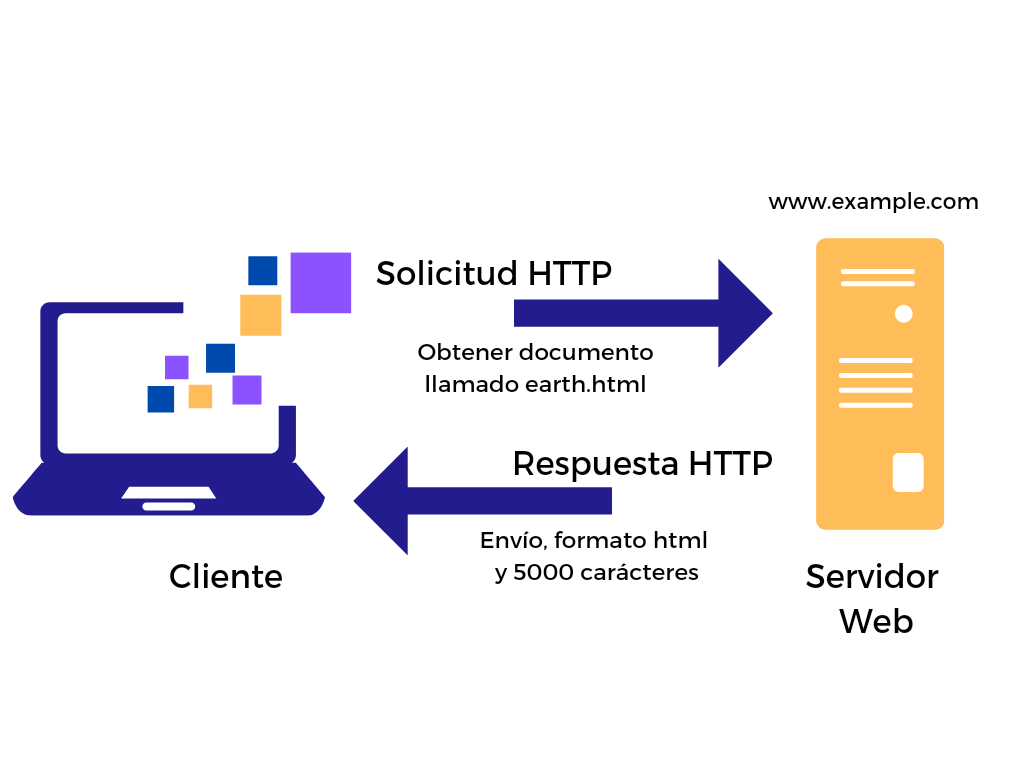
\includegraphics[width=\linewidth]{Cliente-WebServer}
		\caption{Cliente y Servidor Web }
		\label{fig:CSweb}
	\end{figure}
	
	
	\item[Recursos]
	Los servidores web alojan \gls{recursos}. Un recurso web es la fuente del contenido web. El tipo más simple de recurso web es un archivo estático en el sistema de archivos del servidor web: pueden ser archivos de texto, archivos HTML, archivos de Microsoft Word, archivos de Adobe Acrobat, archivos de imagen JPEG, archivos de película AVI o cualquier otro formato, ver Figura \ref{fig:CS-Recursos}..
	Los recursos también pueden ser programas de software que generan contenido bajo demanda. Estos recursos de contenido dinámico pueden generar contenido en función de su identidad, de la información que haya solicitado o de la hora del día, por ejemplo videos, transacciones de comercio electrónico, transacciones bancarias, entre otros
	
		\begin{figure} %
			\includegraphics[width=\linewidth]{Recursos}
			\caption{Clientes, Servidor Web y Recursos }
			\label{fig:CS-Recursos}
		\end{figure}
	

	\item[MIME]
	Debido a que Internet alberga  miles de tipos de datos diferentes, HTTP etiqueta  cada objeto que se transporta a través de la Web con una etiqueta de formato de datos denominada tipo MIME. \gls{MIME} o \textit{Multipurpose Internet Mail Extensions}( en español, Extensiones de correo de Internet multipropósito) se diseñó originalmente para resolver los mensajes entre los sistemas de correo electrónico. HTTP lo adoptó para describir y etiquetar su propio contenido multimedia.

	Los servidores web adjuntan un tipo MIME a todos los datos de objetos HTTP. Cuando un navegador web recupera un objeto de un servidor, mira el tipo MIME asociado para ver si sabe cómo manejar el objeto. La mayoría de los navegadores pueden manejar cientos de tipos de objetos populares: mostrar archivos de imagen, analizar y formatear archivos HTML, reproducir archivos de audio a través de los parlantes de la computadora o iniciar software de complemento externo para manejar formatos especiales, entre otros




	
\end{description}




	
	\begin{itemize}
		\item \texttt{Interacciones de solicitud-respuesta}.  \textit{HTTP} es un \gls{protocolo solicitud-respuesta}.  \textit{HTTP} define un pequeño conjunto de operaciones o métodos que pueden 	realizarse en un recurso. Los más comunes son \textit{GET}, para recuperar datos del recurso y \textit{POST}, para proporcionar datos al recurso.
		
		\item \texttt{Tipos de contenido}. Los navegadores no son necesariamente capaces de manejar todo tipo de contenido. Cuando un navegador realiza una solicitud, incluye una lista de los tipos de contenido que prefiere, por ejemplo, en principio, puede mostrar imágenes en formato \textit{GIF} 		
		pero no en formato \textit{JPEG}. El servidor puede tener esto en cuenta cuando devuelve contenido al navegador. El servidor incluye el tipo de contenido en el mensaje de respuesta para que el navegador sepa cómo procesarlo. El conjunto de las acciones que realizará un navegador para un tipo de contenido determinado son configurables.
		
		\item 	\texttt{Un recurso por solicitud}. Los clientes especifican un recurso por cada  solicitud \textit{HTTP}. Por ejemplo, si una p\'agina web  contiene nueve imágenes,  entonces el navegador emitirá un total de diez solicitudes por separado para la obtención de todo el contenido de la página. Los navegadores suelen hacer varias solicitudes al mismo tiempo, para reducir la demora general para el usuario.
		
		\item \texttt{Control de acceso simple}.  Ccualquier usuario con conectividad de red a un servidor Web puede acceder a cualquiera de sus recursos publicados de forma predeterminada. Si los usuarios desean restringir el acceso a un recurso,  pueden configurar el servidor para que emita una alerta  a cualquier cliente que lo solicita. El usuario correspondiente debe demostrar que tiene derecho a acceder el recurso, por ejemplo, escribiendo una contraseña.
		
	
	
	
	
	
	 \footnote{Amplie su conocimiento visitando este sitio \href{https://www.w3schools.com/whatis/whatis_http.asp} {What is HTTP}  } presenta estas caracter\'isticas:
	 
	 
	 
	 
	 
	 
	 
	  
	\marginnote[-1cm]{
		\begin{kaobox}[frametitle=HTML ]
			Conozca m\'as de URL visitando este sitio  \url{https://www.w3.org/html/}
		\end{kaobox}
	}
	
	Los tipos de 
	
%	A continuación, se muestra un fragmento típico de texto \textit{HTML}, ver figura \ref{fig:Cou-Fig2}:
	
	
%	\begin{figure}%
%		\includegraphics{Coulouris-Fig2.png}
%		\caption{Texto en HTML. Tomado de \CO }
%		\label{fig:Cou-Fig2}
%	\end{figure}
	
%	Este texto \textit{HTML} se almacena en un archivo al que puede acceder un servidor web, por ejemplo  el archivo \textit{earth.html}. Un navegador recupera el contenido de este archivo de un servidor web, en este caso un servidor en una computadora llamada \textit{www.cdk5.net}. El navegador lee el contenido devuelto por 	el servidor y lo convierte en texto formateado e imágenes distribuidas en una página web de una manera adecuada. Solo el navegador, no el servidor, interpreta el texto \textit{HTML}. 
	
%	Pero  el servidor informa al navegador del tipo de contenido que está devolviendo, para distinguirlo de, por ejemplo, un documento en formato de documento portátil. El servidor puede inferir el contenido escrito cuando reconoce la extensión de nombre de archivo \textit{html}.
	
%	La línea 1 del ejemplo \ref{fig:Cou-Fig2}  identifica un archivo que contiene una imagen  su presentación, mediante su \textit{URL}.
%	Línea 2 a la  5 son directivas para comenzar y finalizar un párrafo, respectivamente. 
%	En las líneas 3 y 4 contienen texto que se mostrará en la página web en el formato de párrafo estándar.
%	La línea 4 especifica un enlace en la página web. Contiene la palabra \textit{Moon}  rodeada 	por dos etiquetas HTML relacionada, $<A$ $HREF...>$  y {$</A>$}. El texto entre estas etiquetas es lo que 	aparece en el enlace tal como se presenta en la página web. 
	
%	El navegador registra la asociación entre el texto que se muestra en el enlace y el URL contenido en la etiqueta {$<A$ $HREF...>$} - en este caso:
	
%	\begin{kaobox}[frametitle= Enlace  URL]
%		Enlace $--->$ \href{http://www.cdk5.net/WebExample/moon.html}{Moon}	
%	\end{kaobox}
	
	Cuando el usuario hace clic en el texto, el navegador recupera el recurso identificado por el URL correspondiente y la presenta al usuario. En el ejemplo, el recurso es un archivo \textit{HTML}  que especifica una página web sobre la Luna.
	
%	\item[{URL}] \index{URL} Los navegadores examinan las \gls{URL}	  para acceder a las correspondientes recursos. A veces, el usuario escribe una \textit{URL} en el navegador, o el  navegador busca la \textit{URL} correspondiente cuando el usuario hace clic en un enlace o selecciona uno de sus marcadores o \textit{bookmarks}.
	
	\marginnote{
		\begin{kaobox}[frametitle=URL ]
			Conozca m\'as de URL visitando este sitio
			\href{https://www.w3.org/TR/url/}{URL}  
		\end{kaobox}
	}
	
	
	Cada \textit{URL}, en su forma completa y absoluta, tiene dos componentes de nivel superior:
	
	
	
	\begin{kaobox}[frametitle=Componentes URL]
		scheme : scheme-specific-identifier
	\end{kaobox}
	
	El primer componente declara qué tipo de \textit{URL} es. Los \textit{URL} son necesarios para identificar una variedad de recursos. Por ejemplo, \textit{mailto: joe@anISP.net}	identifica la dirección de correo electrónico de un usuario; \textit{ftp://ftp.downloadIt.com/software/aProg.exe} identifica
	un archivo que se recuperará utilizando el Protocolo de transferencia de archivos (FTP) en lugar del	protocolo HTTP.  
	
	Las \texttt{URL HTTP} son las más utilizadas para acceder a los recursos utilizando el protocolo estándar HTTP. 
	Una \texttt{URL HTTP} tiene dos funciones principales: identificar qué servidor web mantiene el recurso e identificar cuál de los recursos de ese servidor es necesario.
	
	La Figura \ref{fig:WebServer-Exa} muestra tres navegadores que emiten solicitudes de recursos que son administrados por tres servidores web. El navegador superior está emitiendo una consulta a un motor de búsqueda. El navegador del medio requiere la página predeterminada de otro sitio web. El navegador inferior requiere una p\'agina web  que se especifica en su totalidad, incluido un nombre de ruta relativo al servidor.  
	
	\index{DNS}	En general, las \texttt{URL HTTP} tienen el siguiente formato, ver figura \ref{fig:Cou-Fig3}:
	
	\begin{figure}%
		\includegraphics{Coulouris-Fig3.png}
		\caption{ Formato de los URL. Tomado de \CO }
		\label{fig:Cou-Fig3}
	\end{figure}
	
	donde los elementos entre corchetes son opcionales. Una\texttt{ URL HTTP} completa siempre comienza con cadena \textit{http: //} seguida de un nombre de servidor, expresado como un sistema de nombres de dominio (DNS). Opcionalmente, el nombre \gls{DNS} del servidor va seguido del número del puerto en el que el servidor escucha las solicitudes,  el puerto 80 por 	defecto. Luego viene un nombre de ruta opcional del recurso del servidor. Si esto está ausente entonces se requiere la página web predeterminada del servidor. Finalmente, la URL termina opcionalmente en una consulta. 
	
	
	\begin{figure}
		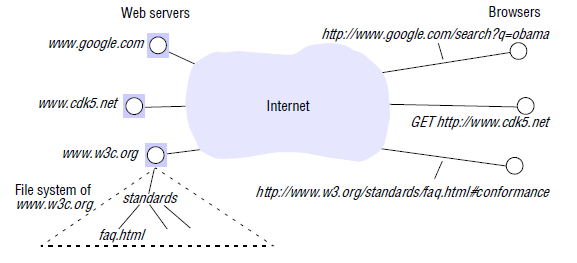
\includegraphics{Coulouris-WebServer.png}
		\caption{Ejemplo de Web Server y Web Browser. Tomado de \CO}
		\label{fig:WebServer-Exa}
	\end{figure}
	
	\item[{HTTP}] \index{HTTP} El Protocolo de transferencia de hipertexto, \gls{HTTP} \footnote{Amplie su conocimiento visitando este sitio \href{https://www.w3schools.com/whatis/whatis_http.asp} {What is HTTP}  } presenta estas caracter\'isticas:
	
	\begin{itemize}
		\item \texttt{Interacciones de solicitud-respuesta}.  \textit{HTTP} es un \gls{protocolo solicitud-respuesta}.  \textit{HTTP} define un pequeño conjunto de operaciones o métodos que pueden 	realizarse en un recurso. Los más comunes son \textit{GET}, para recuperar datos del recurso y \textit{POST}, para proporcionar datos al recurso.
		
		\item \texttt{Tipos de contenido}. Los navegadores no son necesariamente capaces de manejar todo tipo de
		contenido. Cuando un navegador realiza una solicitud, incluye una lista de los tipos de contenido que prefiere, por ejemplo, en principio, puede mostrar imágenes en formato \textit{GIF} 		
		pero no en formato \textit{JPEG}. El servidor puede tener esto en cuenta cuando devuelve contenido al navegador. El servidor incluye el tipo de contenido en el mensaje de respuesta para que el navegador sepa cómo procesarlo. El conjunto de las acciones que realizará un navegador para un tipo de contenido determinado son configurables.
		
		\item 	\texttt{Un recurso por solicitud}. Los clientes especifican un recurso por cada  solicitud \textit{HTTP}. Por ejemplo, si una p\'agina web  contiene nueve imágenes,  entonces el navegador emitirá un total de diez solicitudes por separado para la obtención de todo el contenido de la página. Los navegadores suelen hacer varias solicitudes al mismo tiempo, para reducir la demora general para el usuario.
		
		\item \texttt{Control de acceso simple}.  Ccualquier usuario con conectividad de red a un servidor Web puede acceder a cualquiera de sus recursos publicados de forma predeterminada. Si los usuarios desean restringir el acceso a un recurso,  pueden configurar el servidor para que emita una alerta  a cualquier cliente que lo solicita. El usuario correspondiente debe demostrar que tiene derecho a acceder el recurso, por ejemplo, escribiendo una contraseña.
		
	\end{itemize}
	
	%%	\item[{P\'aginas din\'amicas}]  \index{p\'aginas din\'amicas} Gran parte de la experiencia de los usuarios en la Web es el de interactuar con los servicios en lugar de recuperar datos. Por ejemplo, cuando se compra un artículo en una tienda en línea, el usuario  completa un \gls{formulario web} para proporcionar datos personales o para especificar  lo que se desea comprar.  Cuando el usuario envía el formulario, el navegador envía una solicitud \textit{HTTP} a un servidor web, que contiene los valores que el usuario ha ingresado.
	
	%%%	Dado que el resultado de la solicitud depende de la entrada del usuario, el servidor debe procesar la entrada del usuario. Por lo tanto, la \textit{URL} o su componente inicial designa un 	programa en el servidor. 	Si la entrada del usuario es un conjunto  pequeño de 	parámetros,  se envía como el componente de consulta de la \textit{URL}, utilizando m\'etodo \textit{GET} o alternativamente, se envía como datos adicionales en la solicitud utilizando el m\'etodo \textit{POST}.
	
	%%	Por ejemplo, una solicitud que contiene la siguiente URL invoca un programa llamado búsqueda en \textit{ www.google.com} y especifica una cadena de consulta de \textit{mamul}: 	http://www.google.com/search?q=mamul. 	Ese programa de búsqueda produce texto HTML como salida, y el usuario verá un lista de páginas que contienen la palabra \textit{mamul}.  El servidor devuelve el texto HTML que genera el programa  aunque lo haya recuperado de un archivo. En otras palabras, la diferencia entre el contenido estático  obtenido de un archivo y el contenido  que se genera dinámicamente es transparente para 	el navegador.
	
%	\item[{Servicios Web}] \index{servicios!Web} Otra manera de usar la web es a tr\'aves de los  programas que son clientes de un servicio Web. Sin embargo, \textit{HTML} es inadecuado para la interoperación programática.
	
	
	\marginnote {
		\begin{kaobox}[frametitle=HTML  limitado ]
			Limitado en el sentido de que no es extensible a aplicaciones más allá de la exploración de información,  tiene un conjunto estático de estructuras, y están vinculados con la forma en que los datos se   presentan a los usuarios.
		\end{kaobox}
	}
	
	
%	El lenguaje de marcado extensible, \gls{XML}  ha sido diseñado como una forma de representar datos estandarizados y estructurados,  en formatos espec\'ificos de la aplicaci\'on. Los datos expresados en  ese lenguaje son portables entre aplicaciones ya que es autodescriptivo.
	
	\marginnote [2cm] {
		\begin{kaobox}[frametitle=XML]
			Conozca m\'as de XML visitando este sitio  \href{https://www.w3schools.com/xml/} {XML}
		\end{kaobox}
	}
	
%	En el protocolo \textit{HTTP}, los datos \textit{XML} pueden ser transmitidos por las operaciones \textit{POST} y \textit{GET}.   Por ejemplo, en la tienda de \textit{amazon.com}, las operaciones del servicio web incluyen una para pedir un libro y otra para comprobar
	el estado actual de un pedido.
	
	%	\marginnote {
%		\begin{kaobox}[frametitle=REST ]
			REST   \cite{Fielding2000} adopta este enfoque sobre la base de su extensibilidad: cada recurso en la Web tiene una URL y 	responde al mismo conjunto de operaciones, aunque el procesamiento de las operaciones puede varíar mucho de un recurso a otro.
		\end{kaobox}
		%	} 
	
%	Cualquier operación sobre un recurso puede ser invocado usando uno de los métodos \textit{POST} o \textit{GET}, con contenido estructurado usado para especificar los parámetros, resultados y respuestas de error de la operación. 
	
%\end{description}

%%%%%
